\subsubsection{NDSI Visualization}
The NDSI index measures the relationship between biophony and anthrophony at a site. This is elaborated on in the Overview of Indices section of this report. Because the NDSI is used for comparing two different variables, the representation for this index is different from that of ACI or ADI. Here, two bar charts have been chosen, one for comparing the values per channel, and one for comparing the values side by side. In addition, two line graphs are available for observing the NDSI values along with the biophony and anthrophony for data sets comprised of multiple files, for analyzing these values at their respective time of day.\\

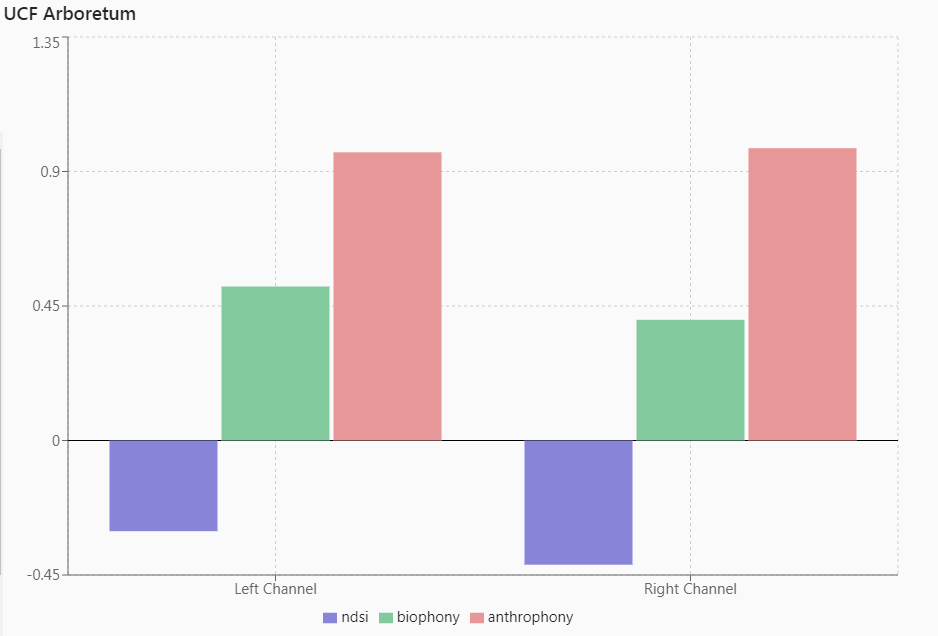
\includegraphics[width=\textwidth]{NDSIgraph1}
The first visualization available is a bar graph comparing the two channels. Each channel has an overall NDSI value, along with biophony and anthrophony values. Because the NDSI is a difference of the anthrophony and biophony, it is useful to view them side by side like so. The user is also able to hover over any bar and see the respective data values as they please.\\

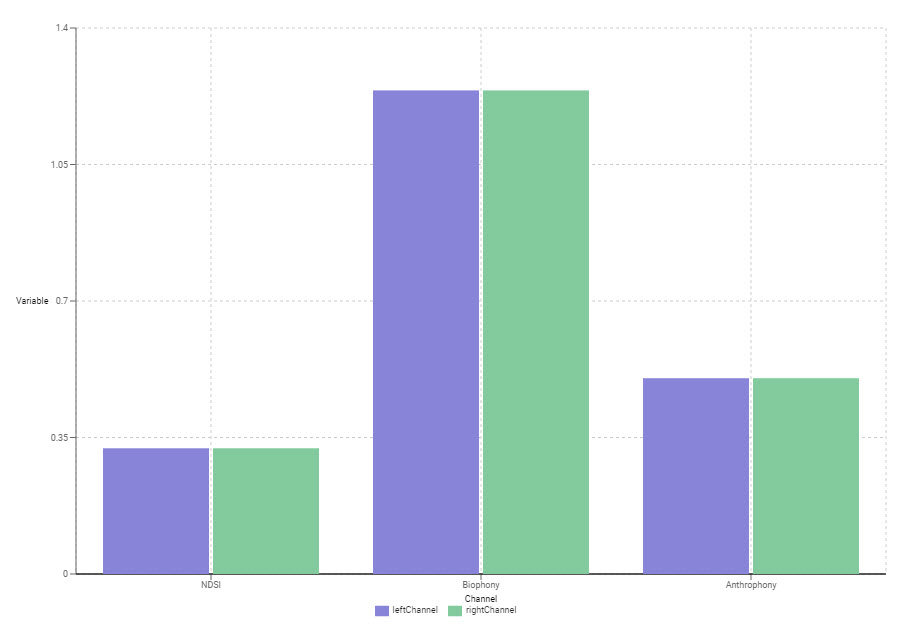
\includegraphics[width=\textwidth]{NDSIgraph2}
The other visualization available is another bar graph, this one showing the NDSI values, anthrophony values, and biophony values side by side, sorted by channel this time. This representation is useful because sometimes one channel of the microphone gets different data outliers than the other, so being able to identify which channel has these outliers is helpful for research.\\

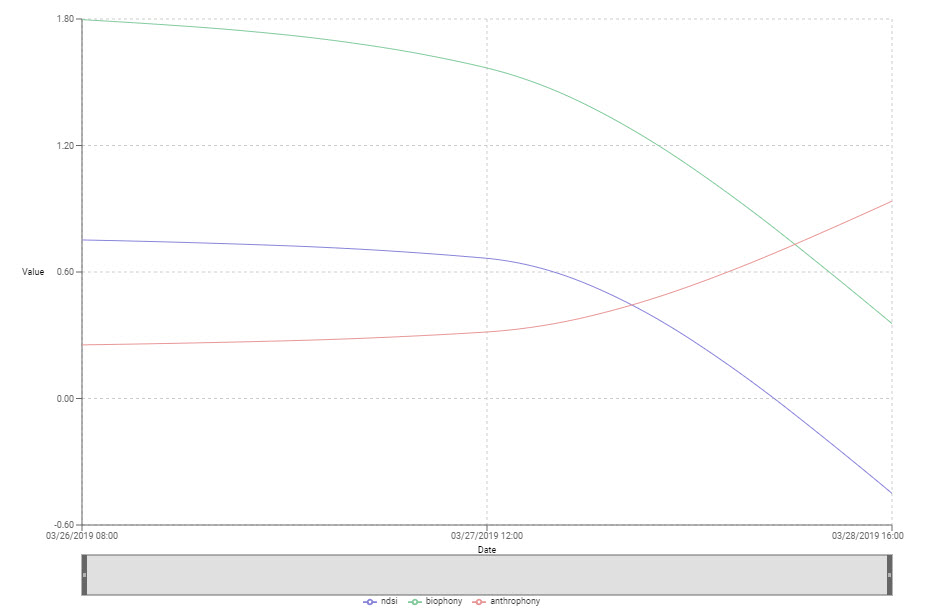
\includegraphics[width=\textwidth]{NDSIgraph3}
The first line graph represents the NDSI value for each channel based on their respective time of day. Researchers often record at different times of day to see how index values compare through out the day.\\

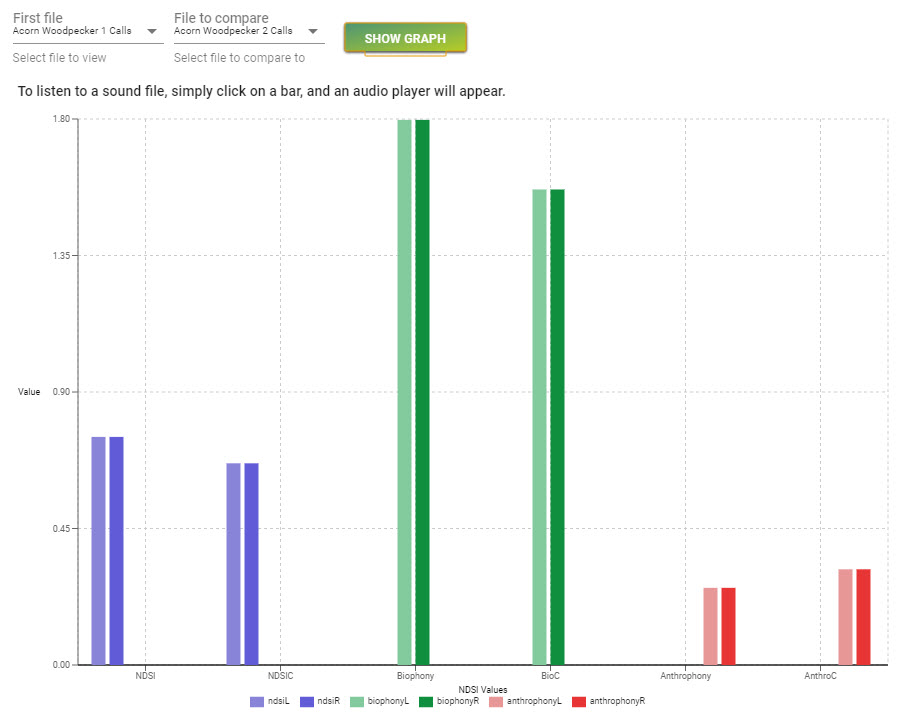
\includegraphics[width=\textwidth]{NDSIgraph4}
And this line graph shows the biophony and anthrophony for each channel, again at different times of day.
